\subsection{Взлом Сапёра при помощи Z3 SMT-солвера}
\label{minesweeper_SMT}

\renewcommand{\CURPATH}{equations/minesweeper_SMT}

Для тех кто не очень хорошо играет в Сапёр (как я), можно предсказывать расположение бомб без помощи отладчика.

Вот я где-то нажал и я вижу пустые ячейки и ячейки с количеством ``соседей'':

\begin{figure}[H]
\centering
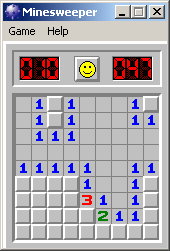
\includegraphics[scale=0.75]{\CURPATH/1.png}
\end{figure}

Что у нас тут, на самом деле? Скрытые ячейки, пустые ячейки (где нет бомб) и пустые ячейки с числами,
показывающими, сколько рядом бомб.

\subsubsection{Метод}

Вот что мы можем сделать: мы будем пытаться расположить бомбу во всех возможных скрытых ячейках и спрашивать Z3 SMT-солвер,
можно ли доказать тот факт, что бомба не может быть расположена там.

Посмотрите на этот фрагмент. "?" означает скрытую ячейку, "." пустую ячейку, число это число соседей.

\begin{center}
\begin{tabular}{ | c | c | c | c | }
\hline
 & C1 & C2 & C3 \\
\hline
R1 & ? & ? & ? \\
\hline
R2 & ? & 3 & . \\
\hline
R3 & ? & 1 & . \\
\hline
\end{tabular}
\end{center}

Так что здесь 5 скрытых ячеек.
Будем проверят каждую скрытую ячейку, располагая там бомбу.
Начинаем с верхней/левой ячейки:

\begin{center}
\begin{tabular}{ | c | c | c | c | }
\hline
 & C1 & C2 & C3 \\
\hline
R1 & * & ? & ? \\
\hline
R2 & ? & 3 & . \\
\hline
R3 & ? & 1 & . \\
\hline
\end{tabular}
\end{center}

Затем мы пытаемся решить следующую систему уравнений (\textit{RrCc} это ячейка из ряда $r$ и столбца $c$):

\begin{itemize}
\item R1C2+R2C1+R2C2=1                               (потому что мы расположили бомбу на R1C1)	
\item R2C1+R2C2+R3C1=1                               (потому что у нас "1" на R3C2)	
\item R1C1+R1C2+R1C3+R2C1+R2C2+R2C3+R3C1+R3C2+R3C3=3 (потому что у нас "3" на R2C2)	
\item R1C2+R1C3+R2C2+R2C3+R3C2+R3C3=0                (потому что у нас "." на R2C3)	
\item R2C2+R2C3+R3C2+R3C3=0                          (потому что у нас "." на R3C3)
\end{itemize}

Как выясняется, эта система уравнений решаема, так что в этой ячейке может быть бомба.
И это информация нам не интересна, так как мы хотим найти ячейки, на которые можно свободно кликать.
И мы попробуем другую.
И если уравнение будет нерешаемо, это будет означать, что там не может быть бомбы, и можно кликнуть.

\subsubsection{Код}

\lstinputlisting{\CURPATH/minesweeper_solver.py}

Этот код самодокументирован и его легко понять без объяснений.
Граница нужна по той же причине, почему реализации игры "Жизнь" Конвея также имеют границу (чтобы сделать
ф-цию для вычисления проще).
Когда мы знаем что в ячейке нет бомбы, мы вписываем туда ноль.
Когда мы знаем количество соседей, мы добавляем констрайнт, снова, как и в игре "Жизнь": количество соседей
должно равняться числу, которое мы увидели в Сапёре.
Затем мы располагаем бомбу где-нибудь и проверяем.

Запускаем:

\begin{lstlisting}
row=1 col=3, unsat!
row=6 col=2, unsat!
row=6 col=3, unsat!
row=7 col=4, unsat!
row=7 col=9, unsat!
row=8 col=9, unsat!
\end{lstlisting}

Это ячейки, которые можно кликать без боязни, что я и сделал:

\begin{figure}[H]
\centering
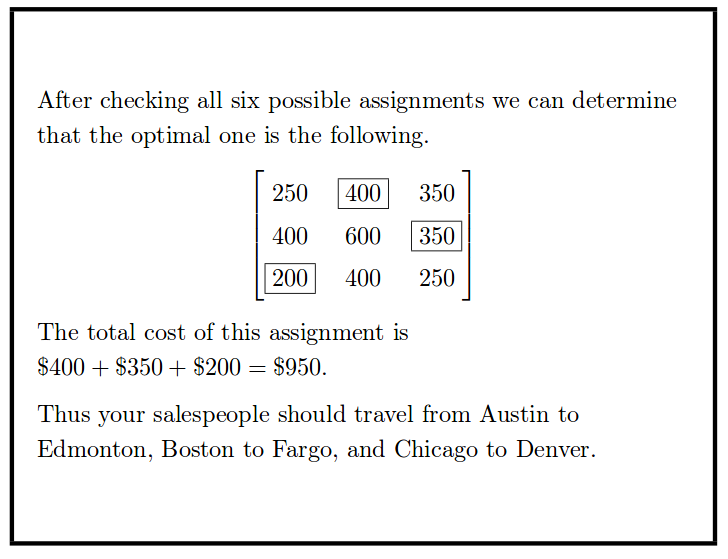
\includegraphics[scale=0.75]{\CURPATH/2.png}
\end{figure}

Теперь у нас больше информации и мы обновляем входное условие:

\begin{lstlisting}
known=[
"01110001?",
"01?100011",
"011100000",
"000000000",
"111110011",
"?11?1001?",
"???331011",
"?????2110",
"???????10"]
\end{lstlisting}

Запускаю снова:

\begin{lstlisting}
row=7 col=1, unsat!
row=7 col=2, unsat!
row=7 col=3, unsat!
row=8 col=3, unsat!
row=9 col=5, unsat!
row=9 col=6, unsat!
\end{lstlisting}

Нажимаю на эти ячейки снова:

\begin{figure}[H]
\centering
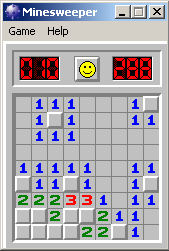
\includegraphics[scale=0.75]{\CURPATH/3.png}
\end{figure}

Обновляю снова:

\begin{lstlisting}
known=[
"01110001?",
"01?100011",
"011100000",
"000000000",
"111110011",
"?11?1001?",
"222331011",
"??2??2110",
"????22?10"]
\end{lstlisting}

\begin{lstlisting}
row=8 col=2, unsat!
row=9 col=4, unsat!
\end{lstlisting}

\begin{figure}[H]
\centering
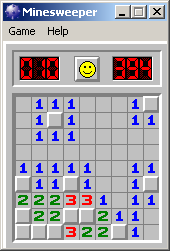
\includegraphics[scale=0.75]{\CURPATH/4.png}
\end{figure}

Последнее обновление:

\begin{lstlisting}
known=[
"01110001?",
"01?100011",
"011100000",
"000000000",
"111110011",
"?11?1001?",
"222331011",
"?22??2110",
"???322?10"]
\end{lstlisting}

\dots последний результат:

\begin{lstlisting}
row=9 col=1, unsat!
row=9 col=2, unsat!
\end{lstlisting}

Вуаля!

\begin{figure}[H]
\centering
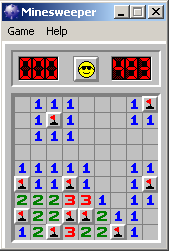
\includegraphics[scale=0.75]{\CURPATH/5.png}
\end{figure}

Исходный код: \url{.../minesweeper_solver.py}.

Обсуждение на HN: \url{https://news.ycombinator.com/item?id=13797375}.

